% Канонический TikZ-рисунок варианта 31. Править только здесь.
\long\def\figStereoV31{%
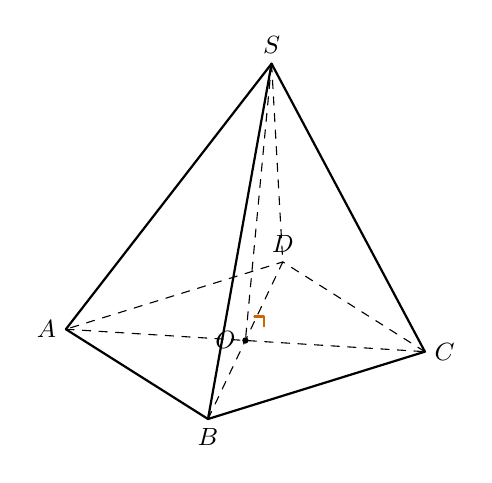
\begin{tikzpicture}[
  scale=0.95,
  line cap=round,
  line join=round,
  every node/.style={font=\small}
]
  % Основание (развёрнуто так, чтобы внутренние линии были лучше видны)
  \coordinate (A) at (-2.6,-0.35);
  \coordinate (B) at (-0.7,-1.55);
  \coordinate (C) at (2.2,-0.65);
  \coordinate (D) at (0.3,0.55);

  % Центр основания
  \coordinate (O) at (-0.2,-0.5);

  % Вершина
  \coordinate (S) at (0.15,3.2);

  % Видимые стороны основания
  \draw[thick] (A)--(B)--(C);

  % Скрытые стороны основания
  \draw[dashed] (C)--(D)--(A);

  % Боковые рёбра
  \draw[thick] (S)--(A);
  \draw[thick] (S)--(B);
  \draw[thick] (S)--(C);
  \draw[dashed] (S)--(D);

  % Диагонали основания
  \draw[dashed] (A)--(C);
  \draw[dashed] (B)--(D);

  % Высота
  \draw[dashed] (S)--(O);

  % Точки
  \fill (O) circle (1.2pt);

  % Значок прямого угла у O
  \draw[orange!80!black, thick]
    (-0.08,-0.18) -- (0.05,-0.18) -- (0.05,-0.31);

  % Подписи
  \node[left]  at (A) {$A$};
  \node[below] at (B) {$B$};
  \node[right] at (C) {$C$};
  \node[above] at (D) {$D$};
  \node[left]  at (O) {$O$};
  \node[above] at (S) {$S$};
\end{tikzpicture}
}
